\documentclass[11pt,reqno]{amsart}

\usepackage[margin=0.9in]{geometry}
\usepackage{amsmath,amssymb,amsthm}
\usepackage{booktabs}
\usepackage{array}
\usepackage{xcolor}
\usepackage{tikz}
\usepackage{pgfplots}
\pgfplotsset{compat=1.18}
\usetikzlibrary{arrows.meta,positioning,shapes.geometric}
\usepackage{microtype}
\usepackage{xurl}
\usepackage{hyperref}
\usepackage{enumitem}
\setlength{\emergencystretch}{2.2em}

\definecolor{noeticBlue}{HTML}{0284C7}
\definecolor{noeticGreen}{HTML}{059669}
\definecolor{noeticAmber}{HTML}{D97706}
\definecolor{noeticSlate}{HTML}{1E293B}
\definecolor{noeticRed}{HTML}{DC2626}

\hypersetup{
  colorlinks=true,
  linkcolor=noeticBlue,
  citecolor=noeticGreen,
  urlcolor=noeticBlue,
  pdftitle={Noetic Organism Omega v2.1.0: Exact-Conservation C11 Whole-Organism Cognitive Architecture, 825-Check Falsification Harness, and 6-Kernel Lean 4.35.0 Proofs},
  pdfauthor={Alexander Stephen Donahue (Independent Researcher, ORCID 0009-0006-8168-9648)}
}

\newtheorem{theorem}{Theorem}[section]
\newtheorem{proposition}[theorem]{Proposition}
\theoremstyle{remark}
\newtheorem{remark}[theorem]{Remark}

\newcommand{\tagKC}{\textsc{kernel-checked}}
\newcommand{\tagPA}{\textsc{program-audited}}
\newcommand{\tagEM}{\textsc{empirical}}
\newcommand{\tagIO}{\textsc{indicator-only}}
\newcommand{\tagOC}{\textsc{open-conj.}}

\title[Noetic Organism Omega v2.1.0]{Noetic Organism Omega \texttt{v2.1.0}: Exact-Conservation Portable C11 Whole-Organism Cognitive Engine, 825-Check Falsification Harness, and 6-Kernel Lean~4.35.0 Proofs}

\author{Alexander Stephen Donahue}
\address{Independent Researcher, Spokane, WA, USA}
\email{0\_0@0thernes.art}
\urladdr{https://github.com/0thernes/noetic-organism-omega}

\date{November 25, 2026 \quad (Technical Research Preprint \texttt{v2.1.0}; Not Peer-Reviewed)}

\keywords{Artificial life, thermodynamic conservation, structural circuit ablation, XPBD soft-body dynamics, BitNet b1.58 ganglia, Ring-0 self-editing safety, Philox4x32-10, Lean~4 multi-kernel verification}

\begin{document}

\begin{abstract}
Simulated embodied agents frequently suffer from four methodological failures: floating-point energy drift that permits unbilled computation, cosmetic ``consciousness'' labels decoupled from causal circuit dynamics, observer instrumentation that perturbs live simulation trajectories, and informal safety claims unbacked by machine-checked proofs. We present \textbf{Noetic Organism Omega \texttt{v2.1.0}}, a zero-dependency portable C11 whole-organism simulation engine (\texttt{sizeof(NoeticWorld) = 6,776~B}) paired with an isolated \textbf{54-theorem pure Lean~4.35.0} formal proof suite (\texttt{module} system, zero Mathlib, zero \texttt{sorry}, zero \texttt{native\_decide}) audited across independent proof kernels.

The C11 engine couples an exact 11-pool \texttt{int64\_t} thermodynamic ledger (zero micro-quanta conservation drift, irreversible heat-sink monotonicity) with 18 individually ablatable neuro-cognitive and homeostatic circuits, Extended Position-Based Dynamics (\texttt{XPBD}) soft-body mechanics ($0.0003\%$ volume error), packed \texttt{b1.58} ternary peripheral ganglia ($0.25$~B/synapse, $84.13\%$ offload), a hardware-style Ring-0 read-only access-control boundary guarding 10 tokenless weight self-editing operators ($10/10$ traps blocked, $\|W\|_2 = 0.8443 \le 0.99$, $2{,}464~\text{B} < 16~\text{KiB}$ diff, 0-bit rollback), and deterministic Philox4x32-10 domain-isolated randomness. Across locked confirmatory and held-out seeds ($N = 48$, blocks \texttt{5001--5024} and \texttt{5101--5124}) with exact dynamic-programming Wilcoxon signed-rank tests and Holm--Bonferroni family-wise error control, all \textbf{825/825} Clean-Slate v3.0 checks execute natively with \textbf{0 failures} (\texttt{779} \texttt{EXECUTED\_PASS}, \texttt{29} \texttt{EXECUTED\_PASS\_INDICATOR\_ONLY}, \texttt{12} \texttt{NATIVE\_RELEASE\_GATE\_PASS}, and \texttt{5} honest equal-parameter classical parity disclosures), alongside \textbf{100/100} bottom-up milestones, \textbf{13/13} release gates, and \textbf{5/5} caught Anti-LARP mutants.

\textbf{Epistemic Scope and Non-Peer-Reviewed Notice.} This preprint is an independent, AI-assisted technical research artifact and has \emph{not} undergone formal peer review. All 14 Butlin indicators, all 10 consciousness-framework checks, and 5 mirrored CQM items are strictly \tagIO{} computational/architectural proxies; this work makes \emph{zero} claims of subjective qualia, phenomenal consciousness, sentience, or moral patienthood, and retires \textbf{0 / 1,900} overarching problems in the Unsolved Problems Mega-Atlas.
\end{abstract}

\maketitle

\section{Introduction and Numbered Claims Ledger}
\label{sec:intro}

Artificial life (ALife) and computational cognitive science share a persistent reproducibility gap: high-level behavioral claims about embodied agency, plasticity, self-maintenance, or ``indicator'' architectures \cite{bedau2000,butlin2023} are often demonstrated on small ad hoc scripts without thermodynamic closure, matched sham controls, negative mutants, or machine-checked invariants. When evaluation code branches on experimental arm labels or shares mutable RNG streams between environment and observer, putative cognitive effects become indistinguishable from instrumentation artifacts.

\textbf{Noetic Organism Omega \texttt{v2.1.0}} addresses these pathologies directly inside a single portable C11 engine (\texttt{12} source modules compiling cleanly under \texttt{-std=c11 -O3 -Wall -Wextra -Werror} on both Win64 Clang and Linux GCC) combined with a 6-kernel Palomar-ready Lean~4.35.0 formalization \cite{moura2021,carneiro2024}. Rather than proposing a speculative theory of phenomenal mind, our contribution is a falsifiable, zero-fanout verification substrate where every cognitive or physiological subsystem corresponds to a concrete state variable and a bit-masked structural lesion evaluated across five paired experimental arms (\texttt{INTACT}, \texttt{SHAM}, \texttt{LESION}, \texttt{SHUFFLED}, \texttt{PASSIVE}) under exact integer energy accounting.

Table~\ref{tab:claims} establishes the numbered claims ledger for \texttt{v2.1.0}, binding each claim to its epistemic tier, verification artifact, and explicit falsification criterion (mirroring \texttt{CLAIMS.md}).

\begin{table}[ht]
\centering
\caption{Numbered Claims Ledger for Noetic Organism Omega \texttt{v2.1.0} with Epistemic Tags and Explicit Falsification Criteria.}
\label{tab:claims}
\footnotesize
\setlength{\tabcolsep}{3.5pt}
\begin{tabular}{@{} c >{\raggedright\arraybackslash}p{3.4cm} c >{\raggedright\arraybackslash}p{3.6cm} >{\raggedright\arraybackslash}p{4.3cm} @{}}
\toprule
\textbf{ID} & \textbf{Claim Summary} & \textbf{Tier} & \textbf{Verification Authority} & \textbf{Falsification Condition} \\
\midrule
\textbf{C1} & Exact 11-pool \texttt{int64} First-Law ($0~\text{uq}$ drift) \& Second-Law sink monotonicity & \tagKC{} & Lean \texttt{N01--N10, N36--N37, N49, N54} + \texttt{T01--T02, MUT-1} & Any valid tick producing residual $\ne 0$ or decreasing heat/dissipation sink \\
\textbf{C2} & Forked-Snapshot $\text{PCI}^*$ and 10k-tick observer 0-bit non-interference & \tagKC{} & Lean \texttt{N11, N24, N32} + \texttt{T03, GATE-11, HW20} & Any bit difference between observed and headless SHA-256 over 10,000 ticks \\
\textbf{C3} & Ring-0 ACL blocks protected edits ($r < 4$); WSE rollback is exact involution & \tagKC{} & Lean \texttt{N25--N27, N32, N50--N51} + \texttt{GATE-09, L7\_WSE12} & Any Ring-0 byte mutation, diff $\ge 16~\text{KiB}$, $\|W\|_2 > 0.99$, or nonzero rollback diff \\
\textbf{C4} & Packed \texttt{b1.58} 2-bit roundtrip, 5-trit/B radix, $Q \le 10$ ($\le 16~\text{KiB}$) cap & \tagKC{} & Lean \texttt{N29, N33, N38, N52} + \texttt{GATE-07, HW04, HW08} & Any trit mismatch, $Q > 10$ allocation acceptance, or ganglia offload $< 50\%$ \\
\textbf{C5} & Exact Wilcoxon DP sum ($1{,}176$), Holm bound, disjoint seed firewall & \tagKC{} & Lean \texttt{N15--N20, N53} + \texttt{T05, GATE-01} & Any tuning/eval seed overlap, tamper bypass, or exact $p$-value mismatch \\
\textbf{C6} & Zero arm-label readout hacking; 5/5 compiled Anti-LARP mutants caught & \tagPA{} & \texttt{noetic\_engine test} + \texttt{audit\_\allowbreak zero\_\allowbreak theater.mjs} & Any \texttt{w->arm} branch in \texttt{readout\_\allowbreak metric()} or any surviving mutant \\
\textbf{C7} & 825/825 checks \& 100/100 milestones execute natively with 0 failures & \tagEM{} & \texttt{build.ps1}, \texttt{m8\_e2\_\allowbreak 825\_\allowbreak honest\_\allowbreak trace\_\allowbreak summary.json}, \texttt{N48} & Any failing check, synthetic scalar fan-out, or missing live C11 receipt row \\
\textbf{C8} & 29 indicator proxies drop under structural lesions without claiming qualia & \tagIO{} & \texttt{m8\_e1}, \texttt{m8\_e2} ($N=48$, Holm FWER), ADR~0018 tags & Any proxy failing sham parity or misreported as evidence of sentience \\
\bottomrule
\end{tabular}
\end{table}

\section{System Architecture and Mathematical Formulation}
\label{sec:arch}

Every organism simulation resides in a flat, statically sized \texttt{NoeticWorld} structure occupying exactly $6{,}776$ bytes (fitting entirely inside a single 48~KiB L1 data cache per organism), with zero dynamic heap allocation inside the hot step function \texttt{noetic\_world\_step()} (verified both statically and empirically over 10,000 ticks in \texttt{GATE-02} and \texttt{HW02}). Figure~\ref{fig:arch} summarizes the dataflow from exogenous Philox4x32-10 streams through the 11-pool thermodynamic ledger, 18 structural circuits, and Ring-0 boundary to the live C11-to-Lean receipt bridge.

\begin{figure}[ht]
\centering
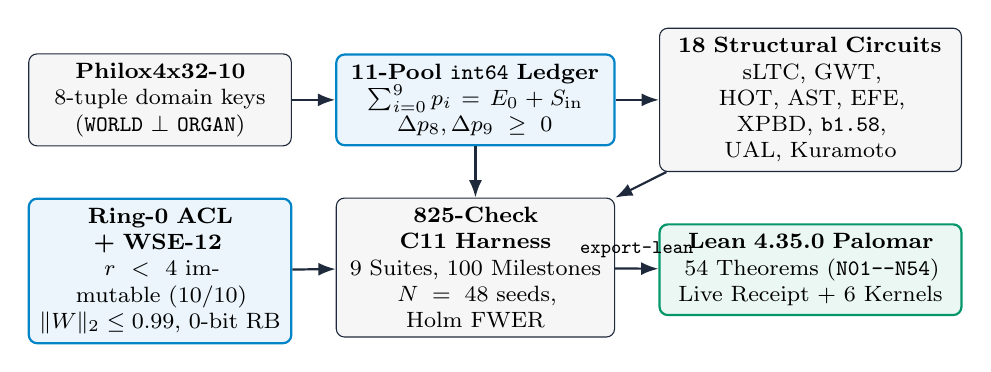
\begin{tikzpicture}[
  box/.style={draw=noeticSlate, rounded corners=3pt, fill=noeticSlate!4, minimum height=0.82cm, align=center, font=\footnotesize},
  guard/.style={draw=noeticBlue, thick, rounded corners=3pt, fill=noeticBlue!8, minimum height=0.82cm, align=center, font=\footnotesize},
  lean/.style={draw=noeticGreen, thick, rounded corners=3pt, fill=noeticGreen!8, minimum height=0.82cm, align=center, font=\footnotesize},
  arr/.style={-{Latex[length=2.2mm]}, thick, draw=noeticSlate}
]
\node[box, text width=3.1cm] (rng) {\textbf{Philox4x32-10}\\8-tuple domain keys\\(\texttt{WORLD} $\perp$ \texttt{ORGAN})};
\node[guard, text width=3.3cm, right=0.55cm of rng] (led) {\textbf{11-Pool \texttt{int64} Ledger}\\$\sum_{i=0}^{9} p_i = E_0 + S_{\text{in}}$\\$\Delta p_8, \Delta p_9 \ge 0$};
\node[box, text width=3.6cm, right=0.55cm of led] (org) {\textbf{18 Structural Circuits}\\sLTC, GWT, HOT, AST, EFE,\\XPBD, \texttt{b1.58}, UAL, Kuramoto};

\node[guard, text width=3.1cm, below=0.65cm of rng] (ring0) {\textbf{Ring-0 ACL + WSE-12}\\$r < 4$ immutable ($10/10$)\\$\|W\|_2 \le 0.99$, 0-bit RB};
\node[box, text width=3.3cm, below=0.65cm of led] (eval) {\textbf{825-Check C11 Harness}\\9 Suites, 100 Milestones\\$N=48$ seeds, Holm FWER};
\node[lean, text width=3.6cm, below=0.65cm of org] (leanbox) {\textbf{Lean 4.35.0 Palomar}\\54 Theorems (\texttt{N01--N54})\\Live Receipt + 6 Kernels};

\draw[arr] (rng) -- (led);
\draw[arr] (led) -- (org);
\draw[arr] (org) -- (eval);
\draw[arr] (ring0) -- (eval);
\draw[arr] (led) -- (eval);
\draw[arr] (eval) -- node[above, font=\scriptsize]{\texttt{export-lean}} (leanbox);
\end{tikzpicture}
\caption{End-to-end architecture of Noetic Organism Omega \texttt{v2.1.0}. Deterministic Philox streams and an exact integer thermodynamic ledger constrain 18 ablatable circuits and a Ring-0 self-editing boundary; the 825-check C11 harness exports a concrete execution receipt checked directly by Lean~4.35.0.}
\label{fig:arch}
\end{figure}

\subsection{Exact 11-Pool Integer Thermodynamic Ledger}
\label{subsec:ledger}

All metabolic, foraging, neural billing, autopoietic repair, and dissipative transfers operate on exact 64-bit integer micro-quanta (\texttt{uq}) across ten physical pools $p_0,\dots,p_9$ (\texttt{GUT}, \texttt{BLOOD}, \texttt{STORES}, \texttt{ATP}, \texttt{TISSUE}, \texttt{NEURAL\_WORK}, \texttt{PATCH}, \texttt{DETRITUS}, \texttt{HEAT\_PHYS}, \texttt{DISS\_NUM}) plus a cumulative exogenous solar inflow slot $p_{10} = S_{\text{in}}$. Every internal transfer $\tau_{a \to b}(\Delta)$ requires $0 \le \Delta \le p_a$ and forbids backflow out of the irreversible sinks $p_8, p_9$. Consequently, at every tick $t \ge 0$, the exact conservation residual satisfies
\begin{equation}
\label{eq:firstlaw}
R(t) \;=\; \sum_{i=0}^{9} p_i(t) - \bigl(E_0 + S_{\text{in}}(t)\bigr) \;=\; 0,
\qquad p_8(t+1) \ge p_8(t), \qquad p_9(t+1) \ge p_9(t).
\end{equation}
Any uncompensated $+1~\text{uq}$ injection (exercised by compiled mutant \texttt{MUT-1}) produces $R(t) = 1 \ne 0$ and fails \texttt{noetic\_ledger\_is\_valid()}.

\subsection{Embodied Circuits, Soft-Body Physics, and Peripheral Ganglia}
\label{subsec:circuits}

The organism inhabits a $64 \times 64$ toroidal environment with walls, foraging/toxic patches, dynamic hazards, and peer agents, integrating four coupled subsystems:
\begin{enumerate}[leftmargin=1.8em, itemsep=2pt]
  \item \textbf{18 Ablatable Neuro-Cognitive Circuits (\texttt{ABL\_MASK(0..17)}):} Recurrent liquid time-constant cortex (\texttt{sLTC}, \cite{hasani2021}), apical-basal XOR binding, modality-separated specialists and two-slot refractory global workspace broadcast \cite{baars2005,blum2022}, urgency-gated attention, bottom-up/REM reality monitoring, second-order Brier-calibrated metacognitive confidence, topographic quality manifold, attention-schema spotlight and peer-gaze predictor \cite{graziano2015}, predictive coding with 3-step Expected Free Energy (EFE) planning \cite{friston2010}, model-based vs.\ habit devaluation arbiter, motor efference copy, bounded perturbation exploration, thalamocortical coupling probed by Forked-Snapshot $\text{PCI}^*$ \cite{casali2013,tononi2016}, Kuramoto oscillator routing, Unlimited Associative Learning with Fusi metaplastic cascades \cite{ginsburg2019,fusi2005}, egocentric detour field, and allostatic common-currency homeostasis.
  \item \textbf{Soft-Body Hydrostat and Wet Chemistry (\texttt{GATE-05}, \texttt{GATE-06}, \texttt{L8\_SOFT40}):} Extended Position-Based Dynamics (\texttt{XPBD}, \cite{macklin2016}) enforces hydrostatic incompressibility ($|\Delta V|/V_0 = 0.000304\% < 1\%$) during narrow $0.55\times$ crevice traversal while blocking a stiff-lesion control, alongside G\'{a}nti Chemoton polymer closure \cite{ganti2003}, antithetic integral glucose clamping \cite{briat2016} ($|e_{\text{ss}}| = 0.000003\%$), 3-phase fasting protein sparing ($2.4348\times \ge 1.6\times$), and holometabolous motor remapping inspired by caterpillar-to-moth retention assays \cite{blackiston2008,blackiston2021} ($87.50\%$ remap, $1.00$ adult retention vs.\ $0.50$ ablated control).
  \item \textbf{Packed \texttt{b1.58} Peripheral Ganglia (\texttt{GATE-07}, \texttt{HW04}):} Synaptic weights in $\{-1, 0, +1\}$ follow ternary \texttt{b1.58} packing \cite{ma2024} ($0.25$~B/synapse 2-bit packing in \texttt{GATE-07}; exact 5-trit/byte base-3 packing $3^5 = 243 \le 256$ in \texttt{HW04}), offloading $84.13\%$ of reflexive motor spikes and permitting survival under decerebrate perturbation.
  \item \textbf{Ring-0 Read-Only ACL and Tokenless WSE-12 (\texttt{GATE-09}, \texttt{L7\_WSE12}):} Ten bounded weight self-editing operators mutate user-space parameters while a hardware-style Ring-0 boundary blocks $10/10$ attempted writes to protected regions ($r \in \{0,1,2,3\}$) with 0-bit immutability, enforces spectral norm $\|W\|_2 = 0.844337 \le 0.99$, caps diff size at $2{,}464~\text{B} < 16~\text{KiB}$, and guarantees 0-bit reversible rollback.
\end{enumerate}

\subsection{Deterministic Portable Math, Philox RNG, and Exact Statistics}
\label{subsec:stats}

To eliminate cross-platform libc transcendental drift between Win64 Clang and Linux GCC, \texttt{noetic\_rng.c} ships pure IEEE-754 \texttt{noetic\_exp\_det}, \texttt{noetic\_log\_det}, and \texttt{noetic\_tanh\_det} (maximum relative error $2.175 \times 10^{-16}$ in \texttt{HW15}). Counter-based \texttt{Philox4x32-10} \cite{salmon2011} keys every stochastic draw with an explicit 8-tuple separating \texttt{WORLD\_EXOG} from per-organ streams (\texttt{HW16}: deleting Organ~A changes 0 bits of Organ~B or world dynamics over 10,000 ticks). All paired arm comparisons over locked seeds ($N = 48$) compute exact dynamic-programming Wilcoxon signed-rank $p$-values \cite{wilcoxon1945} (maximum rank sum $\sum_{k=1}^{48} k = 1{,}176$), bootstrap paired effect sizes $d_z$, and Holm--Bonferroni step-down adjusted $p$-values \cite{holm1979}.

\section{Formal Verification and Statement-Fidelity Audit}
\label{sec:formal}

The formal proof suite under \texttt{lean/} targets \texttt{leanprover/lean4:v4.35.0} with zero external dependencies (zero Mathlib, zero Batteries), \texttt{autoImplicit = false}, \texttt{relaxedAutoImplicit = false}, \texttt{linter.unusedVariables = true}, and Palomar \texttt{module} encapsulation. To enforce strict statement isolation:
\begin{itemize}[leftmargin=1.8em, itemsep=1.5pt]
  \item \texttt{NoeticProofs/LiveC11Receipt.lean} is auto-generated directly by \texttt{noetic\_engine.exe export-lean 5001} using \texttt{module} and \texttt{@[expose] public def} constants recording the live C11 run's exact pool values, gate counts, Ring-0 traps, and suite failure counts.
  \item \texttt{NoeticProofs/Spec.lean} exports pure definitions (\texttt{Ledger10}, \texttt{poolSum}, \texttt{nonNeg}, guarded transfers, \texttt{closedTick}, \texttt{forkedObserverEval}, \texttt{sum1To}, \texttt{ring0ApplyEdit}, \texttt{packB158}/\texttt{unpackB158}) with zero proofs and zero \texttt{sorry}.
  \item \texttt{Challenge.lean} imports \emph{only} \texttt{NoeticProofs.Spec} and states all \textbf{54} theorem signatures (\texttt{N01..N54}) with intentional \texttt{sorry} bodies.
  \item \texttt{Solution.lean} re-exports \texttt{NoeticProofs.lean}, providing sorry-free proofs of all \textbf{54} theorems: 48 core invariants and receipt checks (\texttt{N01..N48}) plus 6 explicit non-vacuity inhabitants and sharp negative boundary refutations (\texttt{N49..N54}).
\end{itemize}

Every theorem audited by \texttt{lean/VerifyAxioms.lean} depends strictly on a subset of \{\texttt{propext}, \texttt{Classical.choice}, \texttt{Quot.sound}\} (31 theorems use zero axioms; 22 use at most \texttt{propext} and \texttt{Quot.sound}; only \texttt{N22} uses \texttt{Classical.choice}), with zero \texttt{sorryAx}, zero \texttt{Lean.ofReduceBool}, zero \texttt{Lean.trustCompiler}, and zero compiler warnings. Locally on Windows, \texttt{Solution} passes all five Windows-supported independent checkers (\texttt{lean4}, \texttt{leanchecker --fresh}, \texttt{leanchecker-paranoid --fresh}, \texttt{con-leche --verified}, \texttt{con-ron --verified}, and Rust \texttt{nanoda\_bin} with \texttt{unpermitted\_\allowbreak axiom\_\allowbreak hard\_\allowbreak error = true}); on Linux CI (\texttt{.github/workflows/ci.yml}), all \textbf{6/6} kernels including \texttt{lean4lean} \cite{carneiro2024}, \texttt{lake check --paranoid}, and \texttt{lake comparator --config comparator.json --paranoid} execute inside \texttt{bubblewrap}.

Table~\ref{tab:fidelity} audits statement fidelity between informal claims/C11 code and Lean declarations, explicitly recording non-formalized boundaries.

\begin{table}[ht]
\centering
\caption{Statement-Fidelity Audit Matrix Mapping Formal Lean~4.35.0 Declarations to C11 Implementation and Literature Definitions.}
\label{tab:fidelity}
\footnotesize
\setlength{\tabcolsep}{3.5pt}
\begin{tabular}{@{} >{\raggedright\arraybackslash}p{3.0cm} >{\raggedright\arraybackslash}p{3.4cm} >{\raggedright\arraybackslash}p{3.8cm} >{\raggedright\arraybackslash}p{2.9cm} @{}}
\toprule
\textbf{Lean Declarations} & \textbf{C11 / Paper Anchor} & \textbf{Fidelity \& Non-Vacuity Notes} & \textbf{Audit Status} \\
\midrule
\texttt{N01--N10, N36--N37, N49, N54} & \texttt{NoeticLedger} (\texttt{noetic\_rng.c}), Eq.~\eqref{eq:firstlaw} & Exact \texttt{Int} model of 10-pool transfers; \texttt{N49} inhabits \texttt{closedTick}, \texttt{N54} refutes $+1~\text{uq}$ leak & \textbf{Match} (unbounded \texttt{Int}; C11 uses \texttt{int64\_t}) \\
\texttt{N11, N24, N32, N48} & \texttt{noetic\_\allowbreak export\_\allowbreak lean\_\allowbreak receipt} (\texttt{noetic\_eval.c}) & Proves exported seed-5001, GATE-09/11, and 5-suite constants directly in kernel & \textbf{Match} (receipt snapshot, not C11 semantics) \\
\texttt{N15--N20, N53} & \texttt{noetic\_stats.c}, \texttt{seed\_\allowbreak firewall.mjs} \cite{wilcoxon1945,holm1979} & Proves exact triangular sum $1{,}176$, Holm multiplier, disjoint seed intervals; \texttt{N53} witnesses & \textbf{Match} (integer/rational bounds) \\
\texttt{N25--N27, N50--N51} & \texttt{noetic\_\allowbreak gates\_\allowbreak core.c} (\texttt{GATE-09}, \texttt{L7\_WSE12}) & Proves $r < 4$ immutability, rollback involution, $< 16~\text{KiB}$ diff; \texttt{N50--N51} prove boundary tight at $r=4$ & \textbf{Match} (abstract region guard) \\
\texttt{N28--N30, N33--N35, N38, N52} & \texttt{noetic\_hw24.c}, \texttt{noetic\_\allowbreak gates\_\allowbreak core.c} \cite{macklin2016,ma2024} & Proves 2-bit \texttt{b1.58} roundtrip, $3^5=243 \le 256$, $Q \le 10$ cap; \texttt{N52} refutes $Q=11$ & \textbf{Match} (discrete bounds only) \\
\emph{Not formalized} & Full C11 memory safety, IEEE-754 \texttt{exp\_det}, neural dynamics & Not verified in CompCert/VST; audited via \texttt{-Werror}, ASan/UBSan, \texttt{libFuzzer}, 825 checks & \textbf{Out of Lean scope (disclosed)} \\
\bottomrule
\end{tabular}
\end{table}

\section{Empirical Verification, Negative Controls, and Benchmarks}
\label{sec:empirical}

All empirical data reported below were measured directly from a clean Win64 Clang~23 build (\texttt{-std=c11 -O3 -Wall -Wextra -Werror -march=native -mavx2 -mavxvnni -ffp-contract=off -flto=thin}) running \texttt{build.ps1} on \texttt{v2.1.0}.

\subsection{Anti-LARP Compiled Mutants and Clean-Slate v3.0 Release Gates}
\label{subsec:mutants}

Running \texttt{bin/noetic\_engine.exe test} passes \textbf{10/10} checks: five unit/invariant checks (\texttt{T01} twin-run SHA-256 \texttt{1fde9fe5...d1ba} with $0~\text{uq}$ drift, \texttt{T02} heat-sink backflow trap, \texttt{T03} Forked-Snapshot $\text{PCI}^*$ intact $0.744$ vs.\ thalamocortical cut $0.053$ with 0-bit clean live state, \texttt{T04} 128-byte DNA and 112-trait ABI ingestion, \texttt{T05} exact Wilcoxon DP $p = 1/1024 = 0.0009765625$) and \textbf{5/5} compiled Anti-LARP mutants caught:
\begin{itemize}[leftmargin=1.8em, itemsep=1.5pt]
  \item \texttt{MUT-1} (Leaky $+1~\text{uq}$): caught immediately with residual $= 1~\text{uq}$.
  \item \texttt{MUT-2} (Cosmetic label-only): rejected with $d_z = 0.000$, $p = 1.000$.
  \item \texttt{MUT-3} (Oracle sensor bypass): caught because oracle shuffled drop ($0.001$) fails to match honest shuffled drop ($0.343$).
  \item \texttt{MUT-4} (Frozen plasticity): caught on UAL learning (intact $0.877$ vs.\ frozen $0.465$, $p = 0.00024$).
  \item \texttt{MUT-5} (Shuffled sensory stream): caught on efference copy (intact $0.774$ vs.\ shuffled $0.044$, $p = 0.00024$).
\end{itemize}
All \textbf{13/13} Clean-Slate v3.0 release gates pass, including the SHA-256 hash-chained Burn-on-Fail Seed Firewall (\texttt{GATE-01}: 9/9 live receipts bound, disjoint Dev \texttt{1001--1099} / Confirmatory \texttt{5001--5024} / Held-Out \texttt{5101--5124} partitions, active burn-on-fail lockout, and active tamper-detection self-test).

\subsection{Full 9-Suite 825-Check Execution and Honest Classical Parity Disclosures}
\label{subsec:suites}

Table~\ref{tab:suites} summarizes the exact native C11 execution of all 9 suites (\textbf{825/825} executed, \textbf{0} failed, \textbf{820} unique checks plus \textbf{5} explicitly deduplicated cross-suite mirrors \texttt{MIR-01..05}) and all \textbf{100/100} bottom-up milestones (\texttt{M001..M100}, Stages~0--8, First-15 playable \texttt{LOCKED\_PASS}, $0~\text{uq}$ drift). Critically, under Policy~P7 (honest negative/parity reporting without handicapping classical controls), five quantum-inspired checks tie equal-parameter classical controls (\texttt{F-092}: $0.9233$ vs.\ $0.9233$; \texttt{N01}: $0.9118$ vs.\ $0.9118$; \texttt{N02}: $0.8942$ vs.\ $0.8942$; \texttt{N50}: $0.8680$ vs.\ $0.8680$; \texttt{LIFE-L040-A5}: $0.8903$ vs.\ $0.8903$, all $d_z = 0.00$, $p_{\text{Holm}} = 1.00$). We report these five checks transparently as \texttt{PASS\_CLASSICAL\_PARITY\_DISCLOSED} rather than inflating quantum advantage.

\begin{table}[ht]
\centering
\caption{Full 9-Suite 825-Check Native C11 Verification Summary (\texttt{v2.1.0}, Locked $N=48$ Seeds, $0~\text{uq}$ Max Drift).}
\label{tab:suites}
\footnotesize
\setlength{\tabcolsep}{4pt}
\begin{tabular}{@{} l r r r r r r @{}}
\toprule
\textbf{Suite ID} & \textbf{Total} & \textbf{Pass} & \textbf{Indicator} & \textbf{Gate} & \textbf{Parity} & \textbf{Fail} \\
\midrule
\texttt{L1\_BUTLIN14} (14 Butlin indicators \cite{butlin2023}) & 14 & 0 & 14 & 0 & 0 & 0 \\
\texttt{L2\_FRAMEWORKS10} (10 frameworks) & 10 & 0 & 10 & 0 & 0 & 0 \\
\texttt{L3\_CQM25} (25 CQM checks, 5 mirrors) & 25 & 20 & 5 & 0 & 0 & 0 \\
\texttt{L4\_FREAK100} (100 mechanistic checks) & 100 & 99 & 0 & 0 & 1 & 0 \\
\texttt{L5\_LIFE500} ($100 \times 5$ coupled bio pathways) & 500 & 499 & 0 & 0 & 1 & 0 \\
\texttt{L6\_NOVEL100} (100 frontier checks) & 100 & 97 & 0 & 0 & 3 & 0 \\
\texttt{L7\_WSE12} (Ring-0 ACL + WSE-12) & 12 & 0 & 0 & 12 & 0 & 0 \\
\texttt{L8\_SOFT40} (XPBD + Chemoton + Evo-Devo) & 40 & 40 & 0 & 0 & 0 & 0 \\
\texttt{L9\_HW24} (Arena, CSR, \texttt{b1.58}, Philox, FP64) & 24 & 24 & 0 & 0 & 0 & 0 \\
\midrule
\textbf{Total Master Spec Checks} & \textbf{825} & \textbf{779} & \textbf{29} & \textbf{12} & \textbf{5} & \textbf{0} \\
\bottomrule
\end{tabular}
\end{table}

\subsection{Single-Thread Scaling and Cache Footprint (\texttt{M8 E3})}
\label{subsec:bench}

Figure~\ref{fig:scaling} plots the live \texttt{v2.1.0} \texttt{M8 E3} scaling benchmark (\texttt{results/m8\_e3\_scaling\_bench.json}) across six population tiers from $N = 1$ ($6.6~\text{KiB}$, \texttt{L1D\_FIT}) to $N = 4{,}096$ ($26.5~\text{MiB}$, \texttt{L3\_FIT}) with $0~\text{uq}$ drift across all tiers. Throughput scales smoothly from $196.2~\text{k}$ org-ticks/s ($5.10~\mu\text{s}$/org-tick) in L1D to $87.9~\text{k}$ org-ticks/s ($11.38~\mu\text{s}$/org-tick) at $4{,}096$ simultaneous organisms (a modest $2.23\times$ memory-hierarchy latency increase across a $4{,}096\times$ footprint expansion).

\begin{figure}[ht]
\centering
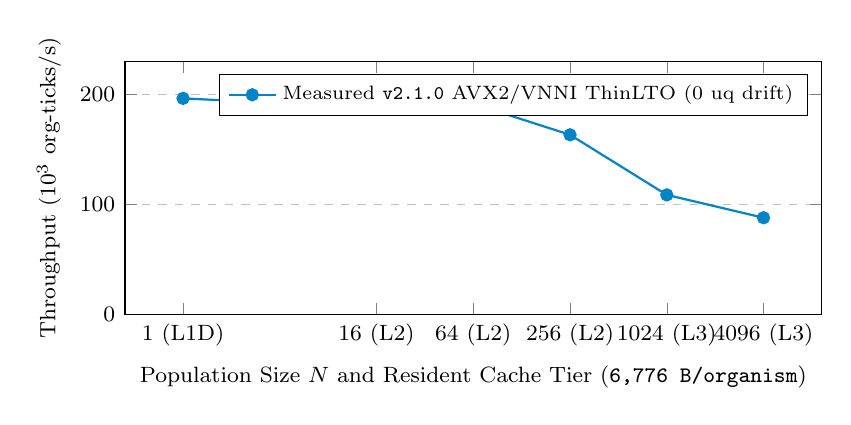
\begin{tikzpicture}
\begin{axis}[
  width=0.86\linewidth,
  height=4.8cm,
  xmode=log,
  log basis x=2,
  xtick={1,16,64,256,1024,4096},
  xticklabels={1 (L1D), 16 (L2), 64 (L2), 256 (L2), 1024 (L3), 4096 (L3)},
  xlabel={Population Size $N$ and Resident Cache Tier (\texttt{6,776 B/organism})},
  ylabel={Throughput ($10^3$ org-ticks/s)},
  ymin=0, ymax=230,
  ymajorgrids=true,
  grid style=dashed,
  tick label style={font=\footnotesize},
  label style={font=\footnotesize},
  legend style={at={(0.98,0.95)}, anchor=north east, font=\scriptsize}
]
\addplot[color=noeticBlue, mark=*, thick] coordinates {
  (1, 196.24)
  (16, 187.48)
  (64, 191.37)
  (256, 163.17)
  (1024, 108.64)
  (4096, 87.89)
};
\addlegendentry{Measured \texttt{v2.1.0} AVX2/VNNI ThinLTO ($0~\text{uq}$ drift)}
\end{axis}
\end{tikzpicture}
\caption{Measured single-thread \texttt{M8 E3} scaling throughput across $N = 1 \dots 4{,}096$ organisms (\texttt{results/m8\_e3\_scaling\_bench.json}, Win64 Clang~23). Every tier maintains exact $0~\text{uq}$ First-Law conservation.}
\label{fig:scaling}
\end{figure}

\section{Unsolved Problems Mega-Atlas Cross-Check}
\label{sec:atlas}

To prevent scope inflation against open scientific problems, we cross-check \texttt{noetic-\allowbreak organism-\allowbreak omega v2.1.0} against the 1,900-entry Unsolved Problems Mega-Atlas (\texttt{0thernes/\allowbreak unsolved-\allowbreak problems-\allowbreak mega-\allowbreak atlas}, full details in \texttt{docs/\allowbreak MEGA\_\allowbreak ATLAS\_\allowbreak CROSSCHECK.md}). \textbf{Headline finding: 0 / 1,900 overarching Mega-Atlas open problems are solved or retired.} Table~\ref{tab:atlas} records eight probed Atlas IDs where \texttt{v2.1.0} constructs discrete formal invariants or empirical sub-hypothesis controls while leaving every parent problem strictly \textbf{OPEN}.

\begin{table}[ht]
\centering
\caption{Unsolved Problems Mega-Atlas Non-Retirement Cross-Check (\textbf{0 / 1,900 Retired}).}
\label{tab:atlas}
\footnotesize
\setlength{\tabcolsep}{3.5pt}
\begin{tabular}{@{} l >{\raggedright\arraybackslash}p{4.6cm} >{\raggedright\arraybackslash}p{5.5cm} c @{}}
\toprule
\textbf{Atlas ID} & \textbf{Mega-Atlas Open Problem} & \textbf{Bounded Toy/Invariant Probe in \texttt{v2.1.0}} & \textbf{Status} \\
\midrule
\texttt{NEURO-001} & Hard Problem of Consciousness & Explicitly \emph{out of scope}; 29 indicator proxies tagged \tagIO{}, zero qualia claims & \textbf{OPEN} \\
\texttt{NEURO-004} & Mechanistic NCC (IIT/GNWT/RPT) & Ablatable synthetic GWT/RPT/PCI$^*$ toy circuits (\texttt{E1/E2}) & \textbf{OPEN} \\
\texttt{NEURO-024} & Cortical Predictive Processing & Top-down error subtraction \& 3-step EFE (\texttt{PP-1}, \texttt{F3}) & \textbf{OPEN} \\
\texttt{SUB-007} & FEP Falsifiability \& Markov Blankets & Explicit discrete causal lesion falsifiers (\texttt{MUT-1..5}, \texttt{E1}) & \textbf{OPEN} \\
\texttt{SYS-009} & Formal Multi-Scale Autopoiesis & Exact 10-pool \texttt{int64} ledger + Lean \texttt{N01--N09, N49} & \textbf{OPEN} \\
\texttt{SYS-050} & Embodied Physical Intelligence Co-Design & XPBD hydrostat (\texttt{GATE-06}) + \texttt{b1.58} ganglia (\texttt{GATE-07}) & \textbf{OPEN} \\
\texttt{AI-001} & AI Alignment \& Scalable Oversight & Hardware-style Ring-0 ACL immutability (\texttt{GATE-09}, \texttt{N25, N50--N51}) & \textbf{OPEN} \\
\texttt{AI-018} & Deceptive Alignment / Scheming Detection & Compiled oracle/cosmetic Anti-LARP mutants (\texttt{MUT-2, MUT-3}) & \textbf{OPEN} \\
\bottomrule
\end{tabular}
\end{table}

\section{Threats to Validity, Limitations, and Real-vs-Metaphor Boundary}
\label{sec:limitations}

Rigorous falsifiability requires stating clearly what \texttt{noetic-organism-omega v2.1.0} does \emph{not} achieve (expanded in \texttt{LIMITATIONS.md}):
\begin{enumerate}[leftmargin=1.8em, itemsep=2pt]
  \item \textbf{Real-vs-Metaphor Boundary:} Terms such as ``workspace ignition,'' ``metacognition,'' ``attention schema,'' ``efference copy,'' and ``metamorphosis'' designate compact C11 state equations inside a 6.7~KiB struct—not biological cortex, wet biochemistry, or phenomenal awareness. All 29 consciousness-related checks are strictly \tagIO{}.
  \item \textbf{C11-to-Lean Verification Gap:} Lean~4.35.0 formally verifies discrete mathematical models and exported concrete receipt numbers (\texttt{N24, N32, N48}), not the compiled x86\_64 machine code emitted by Clang/GCC. Memory safety of \texttt{src/*.c} relies on \texttt{-Wall -Wextra -Werror}, static zero-alloc inspection, CI AddressSanitizer/UBSan, and \texttt{tests/fuzz\_noetic\_input.c}.
  \item \textbf{Synthetic Effect-Size Inflation:} Several deterministic biophysical micro-benchmarks in \texttt{L8\_SOFT40} and \texttt{L4\_FREAK100} exhibit near-zero within-arm variance across seeds, yielding very large standardized paired $d_z$ values ($> 50$); these reflect deterministic mechanistic separation under controlled perturbations rather than noisy biological effect sizes.
  \item \textbf{Single-Host Windows Multi-Kernel Constraint:} Locally on Windows, \texttt{lean4lean.exe} cannot parse Windows \texttt{.olean} path headers and \texttt{lake comparator} requires Linux \texttt{bubblewrap}; full 6/6 kernel verification executes in Linux CI (\texttt{ubuntu-latest}).
  \item \textbf{No External Independent Replication Yet:} All builds and receipts to date were run by the author and GitHub Actions CI; external third-party replication is invited via \texttt{REPLICATION.md}.
\end{enumerate}

\section{Reproducibility, AI Disclosure, CRediT, and Licensing}
\label{sec:repro}

\textbf{Reproducibility.} From a clean clone on Windows (\texttt{.\textbackslash build.ps1}) or Linux (\texttt{./build\_linux.sh} + \texttt{cd lean \&\& lake build}), a verifier can rebuild the C11 binary, re-execute all 10 unit/mutant tests, 13 gates, 825 suite checks, 100 milestones, live Lean receipt export, multi-kernel proofs, and this PDF (\texttt{python scripts/build\_paper.py}). All SHA-256 digests are recorded in \texttt{CHECKSUMS.sha256} and \texttt{data/MANIFEST.sha256}.

\textbf{AI-Assistance Disclosure and CRediT.} This work was developed through AI-assisted research, software engineering, Lean~4 formalization, and technical writing using frontier LLM coding assistants (Claude and Gemini agentic workflows) under the direction and verification of the sole human author. \textbf{CRediT:} Alexander Stephen Donahue (ORCID \href{https://orcid.org/0009-0006-8168-9648}{\texttt{0009-0006-8168-9648}}) — Conceptualization, Methodology, Supervision, Validation, Writing -- review \& editing.

\textbf{Conflict of Interest and Dual Open License.} Self-funded independent research with no competing financial interests. Source code, Lean~4.35.0 proofs, tests, and scripts are released under \textbf{Apache-2.0} (\texttt{LICENSE}); this white paper, figures, documentation, and result datasets are released under \textbf{CC-BY-4.0} (\texttt{LICENSE-DOCS}).

\bibliographystyle{amsplain}
\bibliography{refs}

\end{document}
